\section{Performance}
\iffalse
\begin{frame}{\secname}{Disposition}
    \begin{itemize}
        \item Report Summary
        \item Concurrent Unit Management
        \begin{itemize}
			\item Setup
			\item Results
			\item Discussion
		\end{itemize}
	\end{itemize}
\end{frame}
\fi

\subsection{Report Summary}\label{sec:authors}
\begin{frame}{\secname}{\subsecname}
	.NET Concurrency
	\begin{itemize}
		\item<1-> Lenient mapping to Async Workflows and \texttt{Task}s %up to speed?
		\item<2-> Sequential code faster in binary tree benchmarks
		\item<3-> Concurrent code faster with larger problem sizes:
		\begin{itemize}
			\item 11000-44000 IL instructions in binary tree
			\item Matrix sizes of 512 in matrix summation
		\end{itemize}
		\item<4-> Async Workflow concurrency is fragile
	\end{itemize}
\end{frame}

\begin{frame}{\secname}{\subsecname}
	Unity Technologies advices against functional coding style
	\begin{itemize}
		\item<2-> High order functions
		\item<3-> Closures
		\item<4-> Manipulate existing collections rather than mapping
	\end{itemize}
\end{frame}

\begin{frame}{\secname}{\subsecname}
	Unity Performance - What is Unit Management?
	\inlineMovie[loop&autostart]{unit-management-demo.avi}{pictures/rts-screenshot.png}{width=\textwidth, height=.5625\textwidth}
\end{frame}

\begin{frame}{\secname}{\subsecname}
	Unit Management
	\begin{itemize}
		\item<2-> F\# is marginally slower than C\# in Unity (5-7\% according to \cite{maggiore2012formal,bolhuis2019gameplay})
		\item<3-> FRP system introduces per-\texttt{GameObject} overhead
	\end{itemize}
\end{frame}

\begin{frame}{\secname}{\subsecname}
	Errorneous Code in Inverse Implementation of Unit Management
	\begin{itemize}
		\item<1-> State machine has a list of units.
		\item<2-> When a unit collides with a shot, the unit is added to the list again.
		\item<3-> Many units =\textgreater\ many collisions =\textgreater\ performance degradation.
	\end{itemize}
\end{frame}

\begin{frame}{\secname}{\subsecname}
	Errorneous Code in Inverse Implementation of Unit Management
	\begin{figure}[h!]
		\centering
		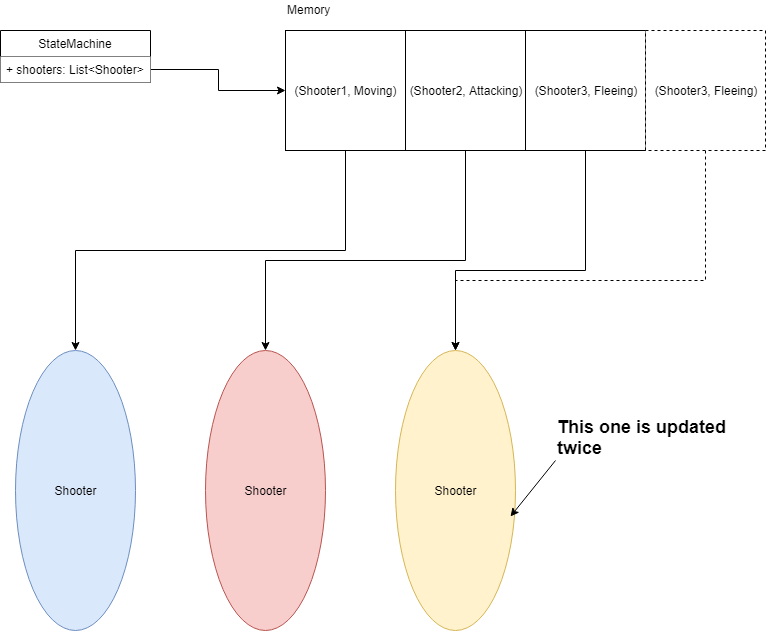
\includegraphics[width=.7\textwidth]{pictures/statemachine.png}
		\caption{Illustration of incorrect implementation of inverse state machine.}
		\label{fig:incorrect:statemachine}
	\end{figure}
\end{frame}

\begin{frame}[fragile]{\secname}{\subsecname}
	Comparison of Errorneous and Correct Implementation
	\barChart[12][\symbolic{Strategy,500,1000,1500,2000,2500}, width=\textwidth,height=.5\textheight][Average FPS][Number of Units]{Comparison of Correct and Errorneous Implementation of Unit Management using the Mono Runtime (higher is better).}{ai:benchmark}{
		\plotData{CSharp Correct}{\sequentialAverageData}
		\plotData{CSharp Incorrect}{\sequentialAverageData}
	}
\end{frame}

\section{Concurrent Unit Management}
\subsection{Setup}
\begin{frame}{\secname}{\subsecname}
	Terminology
	\begin{itemize}
		\item<1-> \texttt{Job} = A definition of how to update a single entity out of a collection. Jobs are executed on worker threads and may be batched.
		\item<2-> \texttt{JobSystem} = A \ttt{MonoBehaviour}, which is in charge of creating and scheduling \texttt{Job}s.
	\end{itemize}
\end{frame}

\begin{frame}{\secname}{\subsecname}
	\begin{itemize}
		\item<1-> Examine if a concurrent implementation of inverse state machine is faster than sequential
		\item<2-> Four \ttt{JobSystem}s:
		\begin{itemize}
			\item Moving Bullets forward
			\item Updating each of the three states (moving, fleeing \& attacking)
		\end{itemize}
		\item<3-> Moving between states sequentially
		\item<4-> Measure the frame rate over 900 frames
	\end{itemize}
\end{frame}

\begin{frame}{\secname}{\subsecname}
	Sequential Implementation
	\begin{figure}[h!]
        \centering
        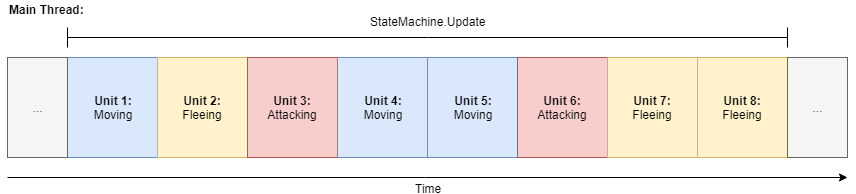
\includegraphics[width=\textwidth]{pictures/sequential.png}
        \caption{A model of sequential execution of inverse state machine.}
    \end{figure}
\end{frame}

\begin{frame}{\secname}{\subsecname}
	Concurrent Implementation
	\begin{figure}[h!]
        \centering
        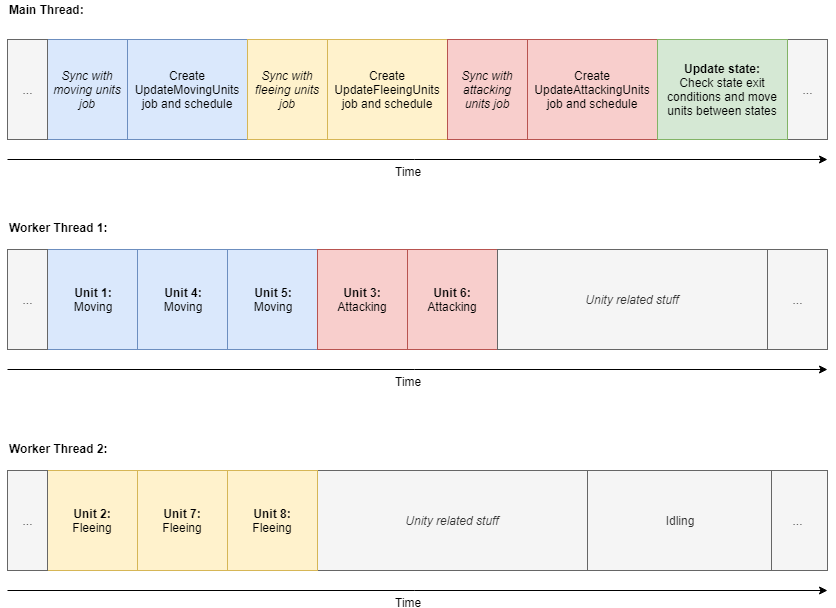
\includegraphics[width=.7\textwidth]{pictures/concurrent.png}
        \caption{A model of concurrent execution of inverse state machine.}
    \end{figure}
\end{frame}

\begin{frame}[fragile]{\secname}{\subsecname}
	Converting from \ttt{JobSystem} representation to \ttt{Job} representation
	\begin{itemize}
		\item<2-> \ttt{JobSystem}s store reference-typed data in lists
		\item<3-> \ttt{Job}s only accept value-type in a \ttt{NativeContainer}s
		\item<4-> Map between representations in each \texttt{Update}
	\end{itemize}
\end{frame}

\begin{frame}{\secname}{\subsecname}
	Converting from \ttt{JobSystem} representation to \ttt{Job} representation
	\begin{figure}[h!]
        \centering
        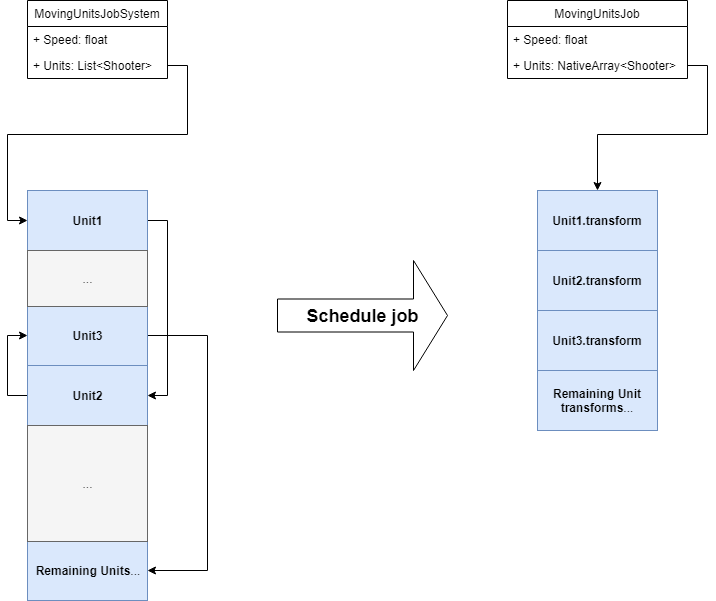
\includegraphics[width=.7\textwidth]{pictures/concurrent-memory-layout.png}
        \caption{Mapping from list of references to array of value-types.}
    \end{figure}
\end{frame}

\begin{frame}{\secname}{\subsecname}
	Test Machine
	\makeTable{{| l | R{6em} | p{3em} |}
	\hline
	\multicolumn{3}{| c |}{\textbf{Processor}} \\ \hline
	Model & \multicolumn{2}{| c |}{Intel Core i7 4702HQ} \\ \hline
	Clock Frequency & 2.2 & GHz \\ \hline
	Max Turbo & 3.2 & GHz \\ \hline
	Physical & 4 & Cores \\ \hline
	Logical & 8 & Cores \\ \hline
	\multicolumn{3}{|c|}{\textbf{Memory}} \\ \hline
	Memory Size & 16 & GiB  \\ \hline
	Memory Speed & 1600 & MHz \\ \hline
	Memory Type &  \multicolumn{2}{| c |}{DDR3L 1600} \\ \hline
	\multicolumn{3}{|c|}{\textbf{Software}} \\ \hline
	Operating System & \multicolumn{2}{| c |}{Ubuntu 18.04 64bit}  \\ \hline
	C\# runtime & \multicolumn{2}{| c |}{dotnet 2.2.104} \\ \hline
	}{System specifications of the test machine.}{sys-specs}
\end{frame}

\subsection{Results}
\begin{frame}{\secname}{\subsecname}
	\begin{itemize}
		\item Concurrent solution is often slower
		\item<2-> Concurrent uses a bit more memory (1500 units):
		\begin{itemize}
			\item Sequential: 1.27Gb
			\item Concurrent: 1.36Gb
		\end{itemize}
	\end{itemize}
\end{frame}

\begin{frame}[fragile]{\secname}{\subsecname}
	Average frame rate over 900 frames
	\barChart[12][\symbolic{Strategy,500,1000,1500,2000,2500}, width=\textwidth, height=.5\textheight][Average FPS][Number of Units]{Average frame rate in the sequential and concurrent implementation of Unit Management (higher is better).}{ai:benchmark:avg}{
		\plotData{Sequential}{\aiAverageData}
		\plotData{Concurrent}{\aiAverageData}
	}
\end{frame}

\begin{frame}[fragile]{\secname}{\subsecname}
	\lineChart[enlarge x limits=false, width=\textwidth, height=.6\textheight, xtick={100,200,300,400,500,600,700,800}][FPS][Frame No.]{FPS for each frame with 500 units (higher is better).}{ai:benchmark:500}{
    \plotUnmarkedData{Sequential 500}{\sequentialData}
    \plotUnmarkedData{Concurrent 500}{\concurrentData}
}
\end{frame}

\iffalse
\begin{frame}[fragile]{\secname}{\subsecname}
	\lineChart[enlarge x limits=false, width=\textwidth, height=.6\textheight, xtick={100,200,300,400,500,600,700,800}][FPS][Frame No.]{FPS for each frame with 1000 units (higher is better).}{ai:benchmark:1000}{
    \plotUnmarkedData{Sequential 1000}{\sequentialData}
    \plotUnmarkedData{Concurrent 1000}{\concurrentData}
}
\end{frame}
\fi

\begin{frame}[fragile]{\secname}{\subsecname}
	\lineChart[enlarge x limits=false, width=\textwidth, height=.6\textheight, xtick={100,200,300,400,500,600,700,800}][FPS][Frame No.]{FPS for each frame with 1500 units (higher is better).}{ai:benchmark:1500}{
    \plotUnmarkedData{Sequential 1500}{\sequentialData}
    \plotUnmarkedData{Concurrent 1500}{\concurrentData}
}
\end{frame}

\begin{frame}[fragile]{\secname}{\subsecname}
	\lineChart[enlarge x limits=false, width=\textwidth, height=.6\textheight, xtick={100,200,300,400,500,600,700,800}][FPS][Frame No.]{FPS for each frame with 2000 units (higher is better).}{ai:benchmark:2000}{
    \plotUnmarkedData{Sequential 2000}{\sequentialData}
    \plotUnmarkedData{Concurrent 2000}{\concurrentData}
}
\end{frame}

\iffalse
\begin{frame}[fragile]{\secname}{\subsecname}
	\lineChart[enlarge x limits=false, width=\textwidth, height=.6\textheight, xtick={100,200,300,400,500,600,700,800}][FPS][Frame No.]{FPS for each frame with 2500 units (higher is better).}{ai:benchmark:2500}{
    \plotUnmarkedData{Sequential 2500}{\sequentialData}
    \plotUnmarkedData{Concurrent 2500}{\concurrentData}
}
\end{frame}
\fi

\subsection{Discussion}
\begin{frame}{\secname}{\subsecname}
	Threats to Validity
	\begin{itemize}
		\item<2-> Experience
		\begin{itemize}
			\item Optimal way of scheduling?
			\item Optimal data representation? (\texttt{NativeArray} instead of \texttt{NativeList})
		\end{itemize}
		\item<3-> Limited generalisability (only tested on one machine)
	\end{itemize}
\end{frame}

\begin{frame}{\secname}{\subsecname}
	Threats to Validity
	\begin{itemize}
		\item A lot of time is spent on Physics
	\end{itemize}
	\begin{figure}[h!]
		\centering
		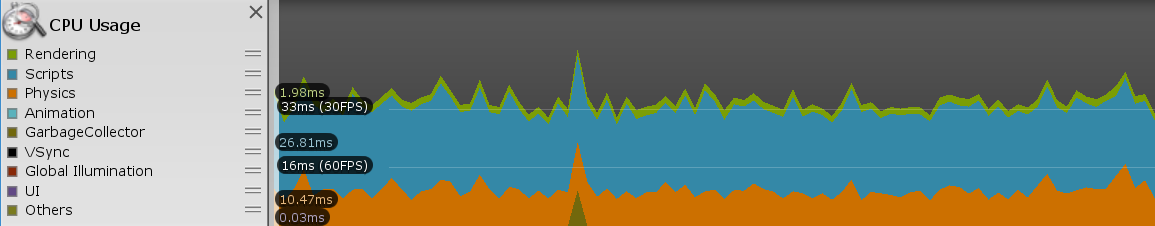
\includegraphics[width=\textwidth]{pictures/profiling.png}
		\caption{CPU utilization output from Unity's Profiler}
		\label{fig:unity:profiler}
	\end{figure}
\end{frame}

\begin{frame}{\secname}{\subsecname}
	Experience with Unity C\# Job System
	\begin{itemize}
		\item<2-> (Almost) writing C++ in C\#
		\begin{itemize}
			\item Manually scheduling \texttt{Job}s
			\item Memory leaks if \texttt{NativeContainer}s are not \texttt{Dispose}d
		\end{itemize}
		\item<3-> No simple way of handling dependencies between \texttt{JobSystem}s
		\item<4-> A lot of converting between representations
		\item<5-> Some expensive operations, such as \texttt{Instantiate} must happen on main thread
		\item<6-> \textbf{A lot of effort for no/limited performance gain}
	\end{itemize}
\end{frame}
